\documentclass{standalone}
\usepackage{tikz}
\usetikzlibrary{shapes,arrows.meta,calc,positioning,decorations.pathmorphing}

% Define colors
\definecolor{MediumSlateBlue}{RGB}{123,104,238}

\begin{document}

% Force-based schematic
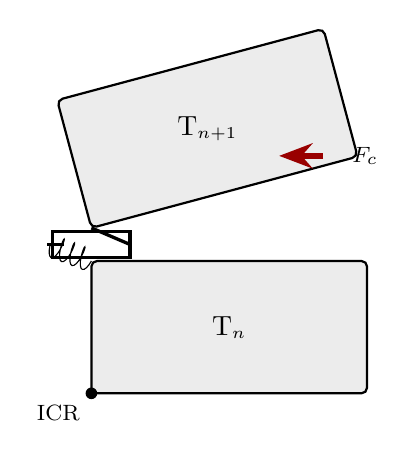
\begin{tikzpicture}[scale=1.4, every node/.style={font=\sffamily, font=\fontsize{8}{8}\selectfont}]
    
    % Setup with realistic proportions
    \def\w{2.5}      % Vertebra width
    \def\h{1.2}      % Vertebra height
    \def\phi{15}     % Rotation angle (used for positioning, not shown)
    
    % Base vertebra Tn
    \coordinate (ICR) at (0,0);
    \coordinate (TnBR) at ($(ICR) + (\w,0)$);
    \coordinate (TnTR) at ($(TnBR) + (0,\h)$);
    \coordinate (TnTL) at ($(ICR) + (0,\h)$);
    
    \fill[gray!15, draw=black, rounded corners=2pt, line width=0.8pt] (ICR) -- (TnBR) -- (TnTR) -- (TnTL) -- cycle;
    \node[font=\sffamily\bfseries, font=\fontsize{9}{9}] at ($(ICR)!0.5!(TnTR)$) {T$_n$};
    
    % Top vertebra Tn+1
    \coordinate (Tnp1BL) at ($(ICR)+(0,\h+0.3)$);
    \coordinate (Tnp1BR) at ($(Tnp1BL) + ({\w*cos(\phi)}, {\w*sin(\phi)})$);
    \coordinate (Tnp1TR) at ($(Tnp1BR) + ({-\h*sin(\phi)}, {\h*cos(\phi)})$);
    \coordinate (Tnp1TL) at ($(Tnp1BL) + ({-\h*sin(\phi)}, {\h*cos(\phi)})$);
    
    \fill[gray!15, draw=black, rounded corners=2pt, line width=0.8pt] (Tnp1BL) -- (Tnp1BR) -- (Tnp1TR) -- (Tnp1TL) -- cycle;
    \node[font=\sffamily\bfseries, font=\fontsize{9}{9}] at ($(Tnp1BL)!0.5!(Tnp1TR)$) {T$_{n+1}$};
    
    % ICR marker
    \fill[black] (ICR) circle (1.5pt);
    \node[below left=1pt] at (ICR) {ICR};
    
    % Spinal cord force vector (behind vertebral bodies)
    \coordinate (cordForceStart) at ($(TnTR)-(0.4,0.1)$);
    \coordinate (cordForceEnd) at ($(Tnp1TR)-(0.4,0.1)$);
    \coordinate (cordForceMid) at ($(cordForceStart)!0.5!(cordForceEnd)$);
    
    % Draw spinal cord force as a thick arrow
    \draw[->, >=Stealth, line width=2pt, color=red!60!black] 
        ($(cordForceMid)+(0.2,0)$) -- ($(cordForceMid)-(0.2,0)$);
    \node[right=5pt] at ($(cordForceMid)+(0.25,0)$) {$F_c$};
    
    % Much larger disc-ligament complex
    \coordinate (discStart) at (TnTL);
    \coordinate (discEnd) at (Tnp1BL);
    \coordinate (discMid) at ($(discStart)!0.5!(discEnd)$);
    
    % Much larger spring-damper representation
    \draw[decorate, decoration={coil,aspect=0.25,segment length=4pt,amplitude=4pt}] 
    (discStart) -- ($(discMid)-(0.4,0)$);
    \draw[line width=1.2pt] ($(discMid)-(0.4,0)$) --++ (0.15,0);
    \draw[line width=1.2pt] ($(discMid)-(0.35,0.12)$) rectangle ++(0.7,0.24);
    \draw[line width=1.2pt] ($(discMid)+(0.35,0)$) -- (discEnd);
    
\end{tikzpicture}

\end{document} 